\documentclass[spanish] {scrartcl}
\setkomafont{disposition}{\normalfont\bfseries}
\usepackage[T1]{fontenc}
\usepackage{selinput}
\usepackage{hyperref}
\usepackage{enumitem}
\usepackage{graphicx}
\SelectInputMappings{%
  aacute={á},
  eacute={é},
  iacute={í},
  oacute={ó},
  uacute={ú},
  ntilde={ñ},
  Euro={€}
}
\usepackage{babel}
\begin{document}
\title{Trabajo Práctico:}
\subtitle{Frank-Hertz}
\author{Gabriel La Torre}
\maketitle
\newpage

\section{Preguntas}

 \begin{enumerate}[label=\alph*)]
    \item Explicar brevemente el experimento de Franck y Hertz (teoría y desarrollo) y su 
significado histórico. ¿Cómo se relaciona el fenómeno de scattering inelástico con la 
excitación de los átomos de mercurio? ¿Es posible ver los fotones generados en las 
desexcitaciones? \\
\\
El experimento de Franck y Hertz consiste en un dispositivo como el de la Figura 1 que emite electrones térmicamente a una energía baja dese el cátodo y son acelerados hacie el ánodo por un potencial aplicado entre los dos electrodos.
	\\\begin{figure}[h]
	  \centering
	    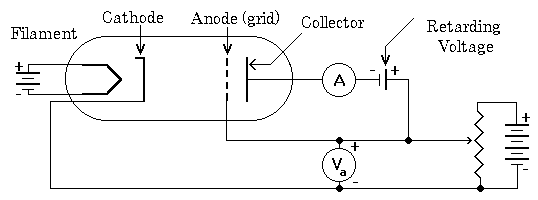
\includegraphics[width=\textwidth]{fhtube}
	  \caption{Experimento de Franck y Hertz}
	  \label{Diagrama del experimento de Franck y Hertz}
	\end{figure}\\

Algunos de los electrones pasan por los agujeros en el ánodo y viajan hacia una placa colectora. Entre la placa y el ánodo hay un pequeño potencial de frenamiento pero la energía cinética con la que los electrones pasan el ánodo es suficiente para vencerla. \\

Durante este proceso los átomos del gas por investigar se encuentran deltro del tubo a una presión baja. Luego se mide la corriente de electrones que llegan a la placa como función del potencial V entre el ánodo y el cátodo, midiendo la corriente con el amperímetro que se ve en la Figura 1.\\
\\
Los resultados de este experimento, realizado en 1914, son la confirmación directo de que los estados de energía interna de un átomo están cuantizados.\\
El fenómeno de scattering que involucra
la experiencia de Franck y Hertz es el de scattering inelástico.
En  este  caso,  los  electrones  transfieren  parte  de  su  energía
cinética  al  átomo,  produciendo  un  estado  de  excitación  del
mismo. \\
Franck y Hertz encontraron que cuando la energía de los electrones de bombardeo es menor que 4.9 eV no se emite ninguna línea espectral del vapor de Hg contenido en el tubo y cuando la energía es un poco mayor solamente se ve una línea en el espectro. La longitud de onda de esta línea es de 2536 \AA, que corresponde exactamente a un fotón de energía de 4.9 eV. En cuanto a si estrictamente es visible, el espectro visible va de 380 a 750 nm y este espectro es de 253,6 nm.\\
  \end{enumerate}


\section{Una fórmula}
Una fórmula con \TeX es mejor:
$$ \frac{\pi}{4} = \int_0^1 \frac{1}{1+x^2} dx $$


http://mate.dm.uba.ar/~pdenapo/tutorial-latex/node2.html

\section{Referencias}

\begin{itemize}
  \item \href{http://www.ib.cnea.gov.ar/~experim2/informes2009/Franck\%20y\%20Hertz\%20Amigo\%20Borda.pdf}{Franck y Hertz - de Amigó-Borda}.
\end{itemize}



\end{document}
